%%%%%%%% ICML 2027 submission skeleton: physical diffusion models with hidden units %%%%%%%%
%
% Skeleton of 2026-11-21. Every section holds bullet points (blue) that say what
% goes there, figure and table placeholders, and result placeholders (red xx.x)
% that are filled in results.tex when the lock-in runs are in.
%
% Compile:  sbatch compile.sh      (or: latexmk -pdf main.tex)
%
% Two switches:
%   \preprintversiontrue   -> arXiv version, authors shown ("Preprint" footer)
%   \preprintversionfalse  -> anonymous ICML submission (the style hides the authors)
%   \shownotesfalse        -> hides the budget notes and TODOs

\documentclass{article}

\newif\ifpreprintversion
\preprintversionfalse          % <- switch here
% compile.sh builds main_preprint.pdf by defining \forcepreprint on the command line
\ifdefined\forcepreprint\preprintversiontrue\fi
\newif\ifshownotes
\shownotestrue                 % <- switch here

% Recommended packages of the ICML template
\usepackage{microtype}
\usepackage{graphicx}
\usepackage{subcaption}
\usepackage{booktabs}
\usepackage{hyperref}
\newcommand{\theHalgorithm}{\arabic{algorithm}}

\ifpreprintversion
  \usepackage[preprint]{icml2027}
\else
  \usepackage{icml2027}
\fi

\usepackage{amsmath}
\usepackage{amssymb}
\usepackage{mathtools}
\usepackage{bm}
\usepackage{enumitem}

% ---------------------------------------------------------------------------
% Skeleton helpers
% ---------------------------------------------------------------------------
\definecolor{plancolor}{RGB}{0,70,140}
\definecolor{tbdcolor}{RGB}{190,0,0}
\definecolor{notegray}{RGB}{110,110,110}

% bullet list that says what goes into a section
\newenvironment{plan}
  {\begin{itemize}[leftmargin=1.1em,itemsep=1pt,topsep=2pt,parsep=0pt]\color{plancolor}}
  {\end{itemize}}
% page budget and open points
\newcommand{\budget}[1]{\ifshownotes{\noindent\small\itshape\textcolor{notegray}{[Budget: #1]}\par}\fi}
\newcommand{\todo}[1]{\ifshownotes\textcolor{tbdcolor}{[TODO: #1]}\fi}
% grey box that stands for a figure
\newcommand{\placeholderbox}[3]{% width, height, text
  \fcolorbox{notegray}{black!5}{%
    \parbox[c][#2][c]{\dimexpr#1-2\fboxsep-2\fboxrule\relax}{\centering\small\color{plancolor}#3}}}

% all numbers of the paper
% =============================================================================
% results.tex -- every number of the paper, one macro per number.
%
% When a run is in, replace \TBD by the value, e.g.
%     \newcommand{\FIDcelebLowExact}{20.20}
% Nothing else in main.tex has to change: the abstract, the text, Table 1 and
% Table 2 all read these macros.
%
% Convention for all FID macros (the locked protocol, 2026-11-21):
%   Inception FID against the train split, noise start, reverse SDE, quench 1,
%   \nSamples generated samples, seed 1.  "Corr" = with two corrector steps.
% =============================================================================

\newcommand{\TBD}{\textcolor{tbdcolor}{\textbf{xx.x}}}

% ---- protocol ----------------------------------------------------------------
\newcommand{\nSamples}{\textcolor{tbdcolor}{\textbf{2{,}000}}} % 2,000 or 10,000: decide
\newcommand{\Slarge}{64}      % sampled hidden states per clamped image, run 2
\newcommand{\Ssmall}{16}      % sampled hidden states per clamped image, run 3
\newcommand{\Kglobal}{16}     % states of the global Potts unit
\newcommand{\Mpatch}{64}      % states of each patch Potts unit
\newcommand{\nSlices}{100}    % time slices

% ---- model size (couplings W + Q per time slice) -----------------------------
\newcommand{\paramsSmall}{\TBD}     % 28x28 (MNIST, Fashion)
\newcommand{\paramsCelebLow}{2.4\,M} % 32x32; notebook 2026-11-21: about 2.4 M
\newcommand{\paramsCelebHigh}{\TBD} % 64x64

% ---- floors: real test images against train, n = 2000 (MODEL_AND_CODE.md) ----
\newcommand{\floorMnist}{3.7}
\newcommand{\floorFashion}{7.2}
\newcommand{\floorCelebLow}{6.4}
\newcommand{\floorCelebHigh}{5.9}

% ---- MNIST, ten digits --------------------------------------------------------
\newcommand{\FIDmnistExact}{\TBD}       % exact statistics, Adam
\newcommand{\FIDmnistSlarge}{\TBD}      % on device, S = 64
\newcommand{\FIDmnistSsmall}{\TBD}      % on device, S = 16
\newcommand{\FIDmnistExactCorr}{\TBD}
\newcommand{\FIDmnistSlargeCorr}{\TBD}
\newcommand{\FIDmnistSsmallCorr}{\TBD}

% ---- Fashion-MNIST, ten classes -----------------------------------------------
\newcommand{\FIDfashionExact}{\TBD}
\newcommand{\FIDfashionSlarge}{\TBD}
\newcommand{\FIDfashionSsmall}{\TBD}
\newcommand{\FIDfashionExactCorr}{\TBD}
\newcommand{\FIDfashionSlargeCorr}{\TBD}
\newcommand{\FIDfashionSsmallCorr}{\TBD}

% ---- CelebA 32x32 grey --------------------------------------------------------
% Exists already: exact, K16 / 64 patch states = 20.20 (Inception job 4287721,
% notebook 2026-11-21). Left as \TBD until the lock-in table is final.
\newcommand{\FIDcelebLowExact}{\TBD}
\newcommand{\FIDcelebLowSlarge}{\TBD}   % running: 4289676, Inception 4289677
\newcommand{\FIDcelebLowSsmall}{\TBD}
\newcommand{\FIDcelebLowExactCorr}{\TBD}
\newcommand{\FIDcelebLowSlargeCorr}{\TBD}
\newcommand{\FIDcelebLowSsmallCorr}{\TBD}

% ---- CelebA 64x64 grey --------------------------------------------------------
\newcommand{\FIDcelebHighExact}{\TBD}
\newcommand{\FIDcelebHighSlarge}{\TBD}
\newcommand{\FIDcelebHighSsmall}{\TBD}
\newcommand{\FIDcelebHighExactCorr}{\TBD}
\newcommand{\FIDcelebHighSlargeCorr}{\TBD}
\newcommand{\FIDcelebHighSsmallCorr}{\TBD}

% ---- sampler ablation, CelebA 32x32 (Table 2) ---------------------------------
\newcommand{\FIDablExactRaw}{\TBD}      % as sampled, no quench
\newcommand{\FIDablSlargeRaw}{\TBD}
\newcommand{\FIDablExactOde}{\TBD}      % probability-flow ODE + quench
\newcommand{\FIDablSlargeOde}{\TBD}
% quench only and quench + corrector reuse \FIDcelebLow... above

% ---- seed spread of the headline model (second wave) --------------------------
\newcommand{\seedSdMnist}{\TBD}
\newcommand{\seedSdFashion}{\TBD}
\newcommand{\seedSdCelebLow}{\TBD}

% ---- earlier models for analog hardware (verify against the papers) -----------
% Wang & Achour, arXiv 2606.27294, their best model; their n and FID code are
% not stated.
\newcommand{\FIDwaMnist}{27.6}
\newcommand{\FIDwaFashion}{80.8}
% DTM and NLM as re-run by Wang & Achour. DTM's own paper (arXiv 2510.23972)
% reports 28 +- 1 on *binarised* Fashion-MNIST; decide which to quote.
\newcommand{\FIDdtmMnist}{107.8}
\newcommand{\FIDdtmFashion}{112.8}
\newcommand{\FIDnlmMnist}{230.5}
\newcommand{\FIDnlmFashion}{200.8}

% ---- compute -------------------------------------------------------------------
\newcommand{\trainHoursExact}{\TBD}     % CelebA 32, one GPU
\newcommand{\trainHoursSlarge}{\TBD}


% notation
\newcommand{\x}{\bm{x}}
\newcommand{\dd}{\mathrm{d}}
\newcommand{\Evis}{E^{\mathrm{v}}}
\newcommand{\gen}{\mathcal{L}}            % generator of the pixel dynamics
\DeclareMathOperator{\Cov}{Cov}

\icmltitlerunning{Physical Diffusion Models with Fast Hidden Units}

\begin{document}

\twocolumn[
  \icmltitle{Physical Diffusion Models with Fast Hidden Units}

  % Author information is removed automatically in the anonymous version.
  \begin{icmlauthorlist}
    \icmlauthor{First Author}{aff}
    \icmlauthor{Second Author}{aff}
    \icmlauthor{Third Author}{aff}
  \end{icmlauthorlist}

  \icmlaffiliation{aff}{Department, University, City, Country}

  \icmlcorrespondingauthor{First Author}{first.author@university.edu}

  \icmlkeywords{physical computing, neuromorphic computing, diffusion models, score matching, local learning, energy-based models}

  \vskip 0.3in
]

\printAffiliationsAndNotice{}

% =============================================================================
\begin{abstract}
% One paragraph. Numbers come from results.tex. ICML asks for 4-6 sentences:
% this has 7, trim when the numbers are in.
Physical systems that generate data through their own stochastic dynamics
promise large savings in energy, but existing proposals are trained by
backpropagation through a digital model, need a second free-running or nudged
phase, or are limited to simple data.
We introduce a score-based diffusion model in which the score is the force of a
physical energy with fast hidden units: a small global Potts unit and Potts units
on overlapping image patches, which sum out exactly and leave the visible units
moving in a free-energy landscape.
Seen as a dense associative memory, its memories are learned at every noise
level instead of stored.
The time-dependent couplings follow a local rule evaluated in a single phase,
with the visible units clamped to data: the thermal fluctuations of the hidden
units supply the response that other physical learning rules obtain from a
second phase.
In simulation, training from \Slarge{} sampled hidden states per data point
reaches an FID of \FIDcelebLowSlarge{} on $32\times32$ CelebA, against
\FIDcelebLowExact{} with exact hidden averages, and the same architecture
generates MNIST, Fashion-MNIST and $64\times64$ faces
(FID \FIDmnistSlarge, \FIDfashionSlarge{} and \FIDcelebHighSlarge).
On MNIST and Fashion-MNIST this improves on earlier generative models designed
for analog hardware.
We describe how each operation of training and generation maps onto analog
crossbar hardware.
\end{abstract}

% ---------------------------------------------------------------- Figure 1 ---
\begin{figure*}[t]
  \centering
  % Source: Conceptual-fig/figure_hidden.tex (compile with Conceptual-fig/compile_fig.sh);
  % frames from Conceptual-fig/make_frames.py.
  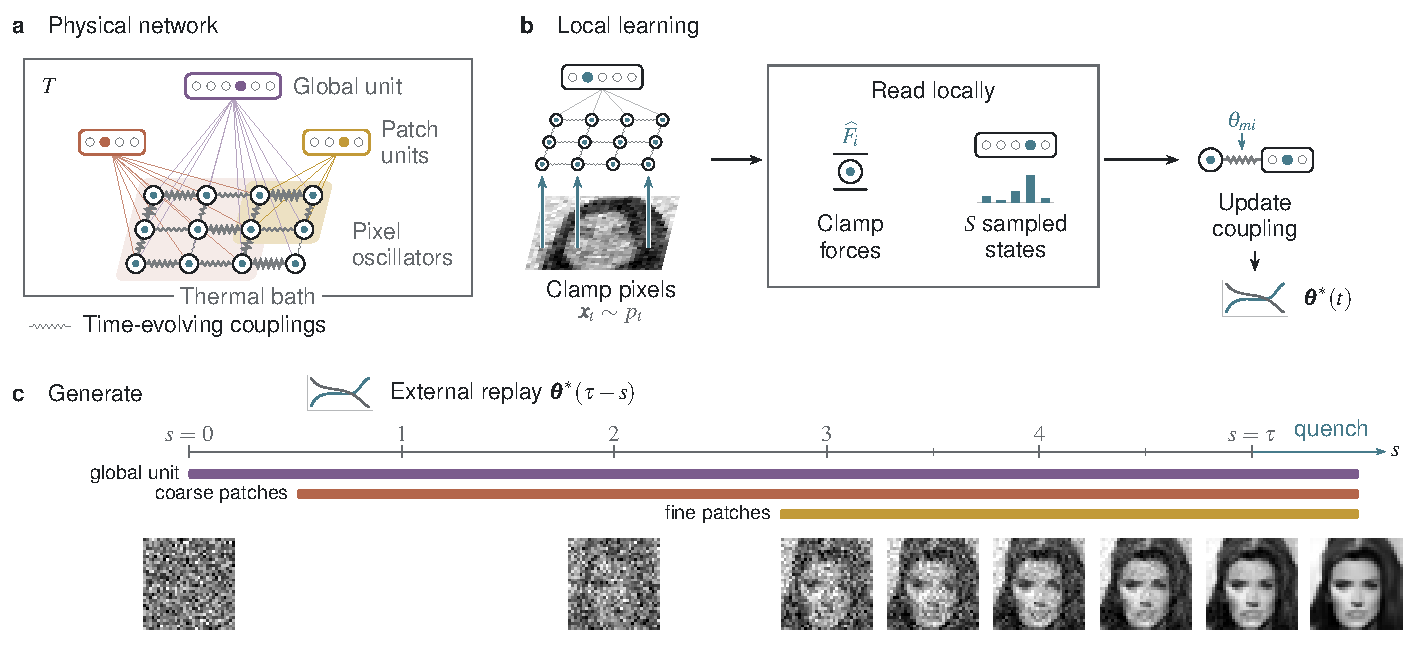
\includegraphics[width=\textwidth]{Conceptual-fig/figure_hidden.pdf}
  \caption{\textbf{A physical diffusion model with fast hidden units.}
    (a)~Pixel oscillators, coupled to their neighbours by springs, interact
    with a thermal bath at temperature $T$. Hidden Potts units (rounded boxes;
    the filled dot is the active state) are coupled to all pixels (global unit,
    purple) or to the pixels of one patch, at a coarse (red) and a fine (yellow)
    scale. They equilibrate fast and are never controlled directly.
    (b)~Learning at one noise level. The pixels are clamped to a noised image
    $\x_t$ and the hidden units settle. Each coupling is updated from quantities
    at its two ends: the clamp force on its pixel and $S$ sampled states of its
    hidden unit. No free-running phase is needed. Repeating this over images and
    noise levels gives the schedule $\bm{\theta}^{*}(t)$.
    (c)~Generation. Starting from noise, an external controller replays
    $\bm{\theta}^{*}(\tau-s)$ in reverse time $s$. The bars, in the colours of
    (a), show when each hidden unit acts: the global unit throughout, the coarse
    patch units from $s\approx0.5$, the fine ones from $s\approx2.8$. A final quench with
    the bath switched off removes the thermal noise. The images are one
    generated $32\times32$ face; the network drawings are schematic.
    \todo{the frames are from the K64 model with 32 patch states: re-render
    from the locked model, and add the frame after the quench.}}
  \label{fig:concept}
\end{figure*}

% =============================================================================
\section{Introduction}
\label{sec:intro}
\budget{0.9 page, including the top of Figure~\ref{fig:concept}}

The energy cost of large generative models has revived interest in hardware
that computes with its own physics: a system whose stochastic dynamics draws
the samples, in place of a processor that simulates such dynamics.
\todo{cite one or two overviews of thermodynamic and physical computing.}
Diffusion models suit this idea. Their reverse process is a Langevin dynamics
in an energy landscape that changes in time
\citep{sohldickstein2015deep,song2021score}, which is what an analog system in
contact with a thermal bath performs when an external schedule drives its
couplings \citep{firstpaper2025}.

Two obstacles remain. The first is expressiveness. An energy made of on-site
potentials and pairwise springs between the visible units can be trained by a
local rule, but it has been shown only on two digit classes of MNIST
\citep{firstpaper2025}. The second is training. More expressive proposals
give up locality or need a second phase. Oscillator networks with hidden units
have been trained adversarially, by backpropagation through a digital solver
\citep{wangachour2026}. Chains of Boltzmann machines subtract a free-running
phase from the clamped one \citep{hinton2002training,jelincic2025dtm}.
Equilibrium propagation compares a free with a nudged equilibrium of the whole
system and gives the gradient in the limit of a vanishing nudge
\citep{scellier2017equilibrium}; it has recently been applied to score, energy
and flow matching
\citep{de2026symmetric,gower2026potentialep,gower2026floweqprop}.

A separate line of work has identified diffusion models with dense
associative memories \citep{krotov2016dense,ramsauer2021hopfield}. The exact
score of a noised training set is the force of a log-sum-exp energy whose
memories are the training images \citep{hoover2023memory,ambrogioni2024search},
and trained networks pass from retrieving these memories to generalising as
the training set grows \citep{pham2026emergence}. Such memories have an analog
circuit: visible and hidden neurons joined by one resistive crossbar, with
hidden neurons that settle faster than the visible ones
\citep{bacvanski2025dense}. But a memory that stores its training set returns
it, and the circuit has been used for retrieval, with weights set by hand or
trained digitally.

Here we join the two lines. We add fast hidden units to a physical diffusion
model in one bipartite layer: a Potts unit coupled to all pixels, Potts units
coupled to overlapping patches at two scales, and one bistable unit per pixel
(Figure~\ref{fig:concept}a). Since the hidden units do not couple to each
other, they sum out exactly. The pixels then move in a free energy whose
gradient is the time-averaged force of the hidden units, and this force,
divided by the temperature, is the score. Our contributions are:
\begin{itemize}[leftmargin=1.3em,itemsep=1pt,topsep=2pt,parsep=0pt]
  \item \textbf{Model.} A dense associative memory at finite temperature, used
        as a diffusion model, whose memories are learned at every noise level:
        a few learned templates per unit in place of the stored training
        images, together with
        local memories on patches (Section~\ref{sec:model}). To our knowledge,
        earlier links between associative memories and diffusion either store
        the data or interpret trained neural networks.
  \item \textbf{Learning rule.} A local rule for the hidden couplings that is
        evaluated in a single phase (Section~\ref{sec:learning}). The pixels
        are fully clamped to data. There is no free-running phase, no nudged
        phase and no limit of small perturbation, because the thermal
        fluctuations of the hidden units carry the response that a nudge would
        measure. The rule follows in a few lines from the generator of the
        pixel dynamics.
  \item \textbf{Results.} Trained from \Slarge{} or \Ssmall{} sampled hidden
        states per clamped image, the model reaches an FID of
        \FIDcelebLowSlarge{} on $32\times32$ CelebA, against
        \FIDcelebLowExact{} with exact hidden averages, and generates MNIST,
        Fashion-MNIST and $64\times64$ faces
        (Section~\ref{sec:experiments}).
        \todo{one clause on the comparison with earlier analog-hardware models
        once the MNIST and Fashion numbers are fixed.}
\end{itemize}
All results are simulations in the limit of fast hidden units. Training
samples the hidden states; the forces at the clamp are computed exactly
(Section~\ref{sec:onephase}). Section~\ref{sec:hardware} discusses the mapping
to hardware.



% =============================================================================
\section{Background: Diffusion as Physical Dynamics}
\label{sec:background}
\budget{0.5 page}

\textbf{Forward process.}
Data $\x_0\in\mathbb{R}^{N}$ are noised by an Ornstein--Uhlenbeck process at
temperature $T$ for $t\in[0,\tau]$,
\begin{align}
  \dd\x &= -\x\,\dd t + \sqrt{2T}\,\dd W , \nonumber\\
  \x_t &= e^{-t}\x_0 + \sqrt{T\,(1-e^{-2t})}\,\bm{\epsilon} ,
  \label{eq:forward}
\end{align}
with $\bm{\epsilon}\sim\mathcal{N}(0,I)$. This is the relaxation of $N$
uncoupled, overdamped harmonic oscillators in a thermal bath, and for
$\tau\gg1$ it ends in their thermal state $\mathcal{N}(0,TI)$. We write $p_t$
for the density of $\x_t$.

\textbf{Score as a force.}
Following \citet{firstpaper2025}, we model $p_t$ by the Boltzmann distribution
of a physical system at the same temperature,
$p_t(\x)\approx e^{-F_t(\x)/T}/Z_t$. The score is then a force divided by the
temperature, $\nabla\log p_t=-\nabla F_t/T$, and the reverse process
\citep{song2021score} reads, in reverse time $s=\tau-t$,
\begin{equation}
  \dd\x = \bigl[\x - 2\nabla F_{\tau-s}(\x)\bigr]\dd s + \sqrt{2T}\,\dd W .
  \label{eq:reverse}
\end{equation}
This is overdamped Langevin dynamics at the bath temperature in the potential
$2F_{\tau-s}(\x)-\tfrac12\lVert\x\rVert^{2}$. Generation is therefore a
physical protocol: prepare the thermal state, then drive the couplings of the
system along a schedule while the bath supplies the noise.

\textbf{Training objective.}
The parameters $\theta$ of $F_t$ are fitted separately at each noise level by
score matching \citep{hyvarinen2005estimation}, which in terms of forces reads
\begin{equation}
  J_t(\theta) = \mathbb{E}_{\x\sim p_t}\!\left[
     -\frac{\Delta F_t(\x)}{T} + \frac{\lVert\nabla F_t(\x)\rVert^{2}}{2T^{2}}
  \right] .
  \label{eq:loss}
\end{equation}
Up to an additive constant, $J_t$ is half the mean squared difference between
the model score $-\nabla F_t/T$ and the score of $p_t$. It needs no samples
from the model. For an energy that is linear in its parameters, such as
on-site potentials and pairwise springs, the gradient of \eqref{eq:loss} is a
sum of local terms measured with the pixels clamped to data
\citep{firstpaper2025}. Such an energy has been shown on two digit classes of
MNIST. It is the baseline that we extend.

% =============================================================================
\section{Model: Fast Hidden Units}
\label{sec:model}
\budget{1.1 pages}

\subsection{Energy and Free Energy}

\textbf{Units.}
Next to the pixels $\x$, the system has discrete hidden units that couple to
the pixels and not to each other (Figure~\ref{fig:concept}a). The building
block is a Potts unit: a hidden unit $u$ with $K_u$ mutually exclusive states.
With state $m$ active, it lowers the energy by its input field
\begin{equation}
  a^{u}_{m}(\x) = b^{u}_{m}
     + \sum_{i\in\mathcal{P}_u}\bigl(W^{u}_{mi}\,x_i + Q^{u}_{mi}\,x_i^{2}\bigr) ,
  \label{eq:field}
\end{equation}
where $\mathcal{P}_u$ is the set of pixels to which the unit is coupled. The
linear coupling $W$ pulls the pixels towards a template, and the quadratic
coupling $Q$ changes their stiffness: for $Q^{u}_{mi}<0$, state $m$ binds pixel
$i$ to the position $-W^{u}_{mi}/2Q^{u}_{mi}$ by a spring of stiffness
$-2Q^{u}_{mi}$. Templates can thus differ in width as well as in position.

We use three kinds of hidden unit:
(i)~one \emph{global} Potts unit with $K$ states, coupled to all pixels;
(ii)~\emph{patch} Potts units with $M$ states each, one for every patch of a
grid of overlapping square patches, in a coarse set and a fine set;
(iii)~one bistable unit $\sigma_i=\pm1$ per pixel, with energy
$-\sigma_i(\nu_i+w_ix_i)$, which can give the pixel an on-site double well.
In our experiments $K=\Kglobal$ and $M=\Mpatch$ (Section~\ref{sec:setup}).
\todo{$K$ on MNIST and Fashion is open: see the outline, section 0.}
The visible energy has the form used by \citet{firstpaper2025}, restricted to
on-site terms and springs between the eight nearest neighbours
$\langle ij\rangle$ of the pixel grid,
\begin{align}
  \Evis_t(\x) ={}& \sum_{i}\Bigl[\tfrac{k_i}{2}x_i^{2}+\tfrac{\lambda_i}{4}x_i^{4}
                   +h_ix_i\Bigr] \nonumber\\
                 & +\sum_{\langle ij\rangle}\kappa_{ij}\,(x_i-x_j)^{2} .
  \label{eq:visible}
\end{align}

\textbf{Summing out the hidden units.}
With $y_u$ the active state of unit $u$, the joint energy is
$E_t=\Evis_t(\x)-\sum_u a^{u}_{y_u}(\x)-\sum_i\sigma_i(\nu_i+w_ix_i)$.
If the hidden units equilibrate much faster than the pixels move, the pixels
feel only the time average of the hidden forces. Because no hidden unit
couples to another, the sum over hidden states factorises, and the pixels move
in the free energy
\begin{align}
  F_t(\x) ={}& \Evis_t(\x)
     - T\sum_{u}\log\sum_{m=1}^{K_u} e^{a^{u}_{m}(\x)/T} \nonumber\\
   & - T\sum_{i=1}^{N}\log 2\cosh\frac{\nu_i+w_i x_i}{T} ,
  \label{eq:free-energy}
\end{align}
where $u$ runs over the global unit and all patch units. A Potts unit spends
the fraction
$p^{u}_{m}(\x)=e^{a^{u}_{m}/T}/\sum_k e^{a^{u}_{k}/T}$
of its time in state $m$ and exerts the force
$G^{u}_{m}=\nabla a^{u}_{m}$ on the pixels while there, with components
$W^{u}_{mi}+2Q^{u}_{mi}x_i$. The gradient of \eqref{eq:free-energy} is the
average of these forces,
\begin{align}
  -\nabla F_t ={}& -\nabla\Evis_t + \sum_{u}\sum_{m}p^{u}_{m}\,G^{u}_{m}
                \nonumber\\
               & + \sum_i w_i\tanh\frac{\nu_i+w_ix_i}{T}\,\bm{e}_i ,
  \label{eq:mean-force}
\end{align}
with $\bm{e}_i$ the unit vector of pixel $i$. The hidden units are neither
controlled nor read during generation.

\textbf{Time dependence.}
Every parameter in \eqref{eq:field}--\eqref{eq:free-energy} depends on the
noise level $t$. The patch sets act only below a noise level of their own: the
coarse set for $t\le t_{\mathrm c}$ and the fine set for
$t\le t_{\mathrm f}<t_{\mathrm c}$, because coarse structure forms at higher
noise than fine detail (Appendix~\ref{app:model-search}). At the highest
noise only the global unit acts.

\textbf{A dense associative memory with learned memories.}
The term of a Potts unit in \eqref{eq:free-energy} is the log-sum-exp energy of
a dense associative memory
\citep{krotov2016dense,demircigil2017model,ramsauer2021hopfield}, in its
formulation with fast hidden neurons \citep{krotov2021large} and at finite
temperature. The model class contains the exact score of the noised training
set $\{\x_n\}_{n=1}^{N_{\mathrm{d}}}$. That density is a mixture of
$N_{\mathrm d}$ Gaussians, which is \eqref{eq:free-energy} with $\Evis=0$ and
one Potts unit with one state per training image:
\begin{equation}
  W_n=\frac{e^{-t}\x_n}{\gamma_t},\quad
  Q_{ni}=-\frac{1}{2\gamma_t},\quad
  b_n=-\frac{e^{-2t}\lVert\x_n\rVert^{2}}{2\gamma_t},
  \label{eq:stored}
\end{equation}
with $\gamma_t=1-e^{-2t}$. This is the memory that
\citet{hoover2023memory}, \citet{ambrogioni2024search} and
\citet{pham2026emergence} identify with a diffusion model; used as a
generator, it returns the training set. We instead keep
$K\ll N_{\mathrm d}$ states and treat $b$, $W$ and $Q$ as parameters, fitted
at every noise level by \eqref{eq:loss}. The patch units add local memories:
$U$ patch units with $M$ states each have $M^{U}$ joint states, so the images
the model can form are not limited to $K$ templates.
With the templates held at data prototypes instead of learned, the same energy
generates far worse images (Appendix~\ref{app:model-search}).
\todo{that comparison (FID 147 against 34 and 22, CelebA $32\times32$) is from
an earlier, larger model: label it so, or repeat it on the locked model.}
In the language of machine learning, each state of a Potts unit is a tilted
copy of the visible model, the global term is a mixture of $K$ such copies,
and the patch units multiply mixtures (Section~\ref{sec:related}).

\textbf{Size.}
The model has \paramsCelebLow{} couplings per noise level at $32\times32$
pixels (\paramsSmall{} at $28\times28$ and \paramsCelebHigh{} at
$64\times64$), nearly all of them in the patch units.
\todo{check ``nearly all in the patch units'' for the final $K$.}

\subsection{Generation}

\textbf{Protocol.}
With $F_t$ fitted, generation runs \eqref{eq:reverse} from
$\x\sim\mathcal{N}(0,TI)$ (Figure~\ref{fig:concept}c). The pixels stay at the
bath temperature, and an external controller replays the couplings
$\theta_{\tau-s}$. We store them at \nSlices{} noise levels and interpolate
linearly in between. The coarse and the fine patch set enter at
$s=\tau-t_{\mathrm c}$ and $s=\tau-t_{\mathrm f}$.

\textbf{The factor two.}
The potential of \eqref{eq:reverse} contains $2F_t$. For the visible energy,
which is linear in its parameters, $2\Evis_t-\tfrac12\lVert\x\rVert^{2}$ is the
same network with other coupling constants. For the hidden units this fails:
doubling the couplings of a unit at temperature $T$ does not double its free
energy, since $-T\log2\cosh(2a/T)\neq-2T\log2\cosh(a/T)$. Two copies of every
hidden unit, each at temperature $T$ and with the trained couplings, give
$2F_t$ exactly, with the whole system at one temperature and all couplings
reciprocal. A gain of two on the force that the hidden units exert on the
pixels gives the same drift without reciprocity
(Appendix~\ref{app:derivation}). Our simulations use the drift of
\eqref{eq:reverse} directly.

\textbf{Quench and corrector.}
After the reverse process we switch the bath off for a short time,
$\dot{\x}=-\nabla F_{0}(\x)$. The pixels relax in the final landscape, which
removes the thermal speckle (Table~\ref{tab:sampler}). Optionally, two Langevin
steps at fixed couplings follow every stored noise level, the corrector of
\citet{song2021score}.

\textbf{Validity.}
The free-energy picture holds if the hidden units equilibrate faster than the
pixels relax and faster than the couplings change
(Appendix~\ref{app:derivation}). Our simulations take this limit: they evaluate
the occupations and the mean force \eqref{eq:mean-force} in closed form and do
not simulate hidden trajectories.

% =============================================================================
\section{Learning from Statistics at Clamped Data}
\label{sec:learning}
\budget{1.0 page planned; about 1.4 with the derivation in the main text}

Throughout this section the pixels are \emph{clamped}: held by an external
constraint at a noised training image $\x\sim p_t$, while the hidden units
equilibrate. We write $\bm{\psi}(\x)=\nabla F_t(\x)$ for the force that the
clamp must supply, and $\langle\,\cdot\,\rangle$ for the average over
$\x\sim p_t$.

\subsection{The Gradient as a Response to Release}

Let $\theta$ be any parameter of $F_t$. Differentiating \eqref{eq:loss} gives
\begin{equation}
  \partial_\theta J_t = -\frac{1}{T^{2}}
     \bigl\langle \gen\,\partial_\theta F_t \bigr\rangle ,
  \qquad
  \gen = T\Delta - \bm{\psi}\!\cdot\!\nabla .
  \label{eq:generator}
\end{equation}
The operator $\gen$ is the generator of the Langevin dynamics of the pixels in
$F_t$: for an observable $g$, $\gen g(\x)$ is the rate at which the mean of
$g$ changes when the pixels are released from $\x$. The observable
$\partial_\theta F_t$ is the Hebbian term of a Boltzmann machine, for example
$-p_m$ for the bias of state $m$ and $-p_mx_i$ for its coupling to pixel $i$.
Equation \eqref{eq:generator} thus says that learning has converged when the
Hebbian terms are stationary under the model's own dynamics started from data.

A device could measure $\gen\,\partial_\theta F_t$ literally, by releasing the
pixels for a short time and reading the Hebbian term before and after. This is
contrastive divergence with one short Langevin step
\citep{hinton2002training,hyvarinen2007connections}. It is a difference of two
noisy readings whose signal vanishes with the release time. We instead
evaluate $\gen\,\partial_\theta F_t$ at the clamp.

\subsection{The Rule for a Potts Unit}

Consider one Potts unit and drop its index $u$. Let
$\bar G=\sum_k p_kG_k$ be the mean force of the unit on the pixels and
$\delta G_m=G_m-\bar G$ the excess force of state $m$. The occupations respond
to a displacement of the pixels as
\begin{equation}
  \nabla p_m = \frac{p_m}{T}\,\delta G_m .
  \label{eq:response}
\end{equation}
Taking the divergence of \eqref{eq:response}, with
$\nabla\!\cdot G_m=2q_m$ and $q_m=\sum_iQ_{mi}$, and inserting both into
$\gen$ gives
\begin{align}
  \gen\,p_m &= \frac{p_m}{T}\,c_m , \qquad
  c_m = \phi_m-\sum_k p_k\phi_k , \nonumber\\
  \phi_m &= \delta G_m\!\cdot\!\bigl(\delta G_m-\bm{\psi}\bigr) + 2T\,q_m .
  \label{eq:cm}
\end{align}
The parameters of state $m$ enter $F_t$ through
$\partial_{b_m}F_t=-p_m$, $\partial_{W_{mi}}F_t=-p_mx_i$ and
$\partial_{Q_{mi}}F_t=-p_mx_i^{2}$. The product rule
$\gen(fg)=f\gen g+g\gen f+2T\,\nabla f\!\cdot\!\nabla g$, together with
$\gen x_i=-\psi_i$ and $\gen x_i^{2}=2T-2x_i\psi_i$, then turns
\eqref{eq:generator} into
\begin{align}
  \partial_{b_m}J_t &= \frac{\langle p_m c_m\rangle}{T^{3}} , \nonumber\\
  \partial_{W_{mi}}J_t &= \Bigl\langle p_m\Bigl[\tfrac{x_i c_m}{T^{3}}
      + \tfrac{2\,\delta G_{mi}-\psi_i}{T^{2}}\Bigr]\Bigr\rangle , \nonumber\\
  \partial_{Q_{mi}}J_t &= \Bigl\langle p_m\Bigl[\tfrac{x_i^{2}c_m}{T^{3}}
      + \tfrac{2x_i(2\,\delta G_{mi}-\psi_i)}{T^{2}}
      + \tfrac{2}{T}\Bigr]\Bigr\rangle .
  \label{eq:rule}
\end{align}
This is the complete rule. With several hidden units, each unit obeys
\eqref{eq:rule} with its own $p$, $G$ and $\phi$ and with the total clamp
force $\bm{\psi}$: the Laplacian in \eqref{eq:loss} is additive over the units,
so no cross terms between units appear. The bistable units are the case of two
states with opposite fields. For a parameter of the visible energy,
$\partial_\theta F_t$ is a fixed function of $\x$ and \eqref{eq:generator} is
the rule of \citet{firstpaper2025}, with $\bm{\psi}$ now including the mean
force of the hidden units. Equation \eqref{eq:rule} agrees with automatic
differentiation of \eqref{eq:loss} to rounding error, on trained models for
the global and per-pixel units and on a small test model that includes patch
units (Appendix~\ref{app:derivation}).

\subsection{One Phase at Full Clamp}
\label{sec:onephase}

\textbf{No second phase.}
Equation \eqref{eq:rule} is one experiment per training image. The pixels are
held at the noised data point, the hidden units equilibrate, and everything is
read at this one configuration. There is no free-running phase as in
Boltzmann learning \citep{hinton2002training,jelincic2025dtm}, no second,
nudged equilibrium of the whole system as in equilibrium propagation
\citep{scellier2017equilibrium}, and no limit of small perturbation. The clamp
is a full clamp, as in the positive phase of a Boltzmann machine; the negative
phase is replaced by higher moments of the hidden units in the positive phase.

\textbf{Fluctuations take the place of the nudge.}
Equation \eqref{eq:response} is a response of the hidden unit to a
displacement of the pixels, which a deterministic unit could only reveal if
the pixels were displaced. A thermal unit reveals it in its fluctuations at
the fixed clamp. As the unit hops between its states $k$, let $\phi_k$ be the
scalar of \eqref{eq:cm} for the state that is active. Then
\begin{equation}
  \gen\,p_m = \frac{1}{T}\,\Cov_k\bigl(\delta_{km},\,\phi_k\bigr) ,
  \label{eq:cov}
\end{equation}
the covariance, over the unit's own thermal states, between ``state $m$ is
active'' and $\phi$. The term of $\phi$ that is linear in $\bm{\psi}$ is the
fluctuation--response relation
$\bm{\psi}\!\cdot\!\nabla p_m=\Cov_k(\delta_{km},G_k\!\cdot\!\bm{\psi})/T$; the
quadratic term comes from the Laplacian in the same way.

\textbf{The rule per read.}
Read the hidden unit $S$ times while the pixels are clamped. If a read finds
the unit in state $k$, only the parameters of that state are updated:
\begin{align}
  \Delta b_k &\propto -\frac{\phi_k-\bar\phi}{T^{3}} , \nonumber\\
  \Delta W_{ki} &\propto -\frac{x_i(\phi_k-\bar\phi)}{T^{3}}
                 -\frac{2\,\delta G_{ki}-\psi_i}{T^{2}} ,
  \label{eq:per-read}
\end{align}
and likewise for $Q_{ki}$, where $\bar\phi$, $\bar G$ and $\bm{\psi}$ are
averages over the $S$ reads. Averaged over the reads, \eqref{eq:per-read} is
\eqref{eq:rule} with the occupations $p_m$ replaced by the measured
frequencies $\hat p_m$. A coupler $(k,i)$ needs one scalar of its hidden state,
$\phi_k-\bar\phi$, and signals of its pixel: the position $x_i$, the clamp
force $\psi_i$, and the excess force $\delta G_{ki}$ that the unit exerts on
this pixel during the read.

\textbf{What a device measures.}
(i)~The active state of every hidden unit at each read.
(ii)~The time-averaged force on every clamp, $\psi_i$.
(iii)~The sum over the unit's pixels inside $\phi_k$, the only quantity that
is not local to a coupler. It can be accumulated along the unit's line, or
read from the unit's input field under symmetric pairs of probe displacements
$\pm\varepsilon\bm{v}$ of the clamp:
$[a_k(\x+\varepsilon\bm{v})-a_k(\x-\varepsilon\bm{v})]/2\varepsilon
=G_k\!\cdot\!\bm{v}$
holds for any $\varepsilon$, because the fields are quadratic in $\x$
(Appendix~\ref{app:derivation}). Such a probe reads an inner product. It
carries no error signal and is not a second phase.

\textbf{The price.}
First, the hidden units must be thermal. A deterministic element with output
$p_m$ has no fluctuations to read, and its response would have to be measured
by displacing the clamp. Second, \eqref{eq:rule} contains products of
measured averages, so its estimate from $S$ reads is biased at order $1/S$.
This bias takes the place of the finite-nudge bias of equilibrium propagation,
and Section~\ref{sec:sampled} removes it. Third, in our simulations only (i)
is sampled: the clamp forces and the sums over pixels are computed in exact
arithmetic from the sampled states, without read noise.

\subsection{Sampled Hidden Statistics}
\label{sec:sampled}

\textbf{Jackknife.}
Let $\hat J_S$ be the loss \eqref{eq:loss} with every occupation replaced by
its frequency over $S$ reads. The loss is quadratic in these frequencies, and
\begin{equation}
  \mathbb{E}\bigl[\hat J_S\bigr] = J_t - \frac{V}{2ST^{2}} ,
  \label{eq:bias}
\end{equation}
where $V$ is the variance of the forces that the hidden units exert on the
pixels, summed over all hidden units and averaged over the data. We remove
this bias, and the bias of the gradient to first order in $1/S$, with a
jackknife over the same reads, using the loss of all $S$ reads and of its two
halves,
\begin{equation}
  \hat J^{\,\mathrm{jk}}_S = 2\hat J_S
    -\tfrac12\bigl(\hat J^{(1)}_{S/2}+\hat J^{(2)}_{S/2}\bigr) ,
  \label{eq:jackknife}
\end{equation}
which costs no further reads. On a device, this means averaging the hidden
read-outs over one full window and its two halves
(Appendix~\ref{app:sampled}).

\textbf{Visit-count rule.}
With few reads, a rarely occupied state is rarely visited. Its gradient is
zero in most steps and large in the others, and an optimiser that normalises
every coupling by its own gradient history, such as Adam
\citep{kingma2015adam}, then moves it too slowly and the state dies out. For
the hidden couplings we therefore keep, per state, a leaky average of its
gradient and a leaky count of its visits, and step by their ratio
(Appendix~\ref{app:sampled}). This needs one counter per hidden state.

% =============================================================================
\section{Experiments}
\label{sec:experiments}
\budget{3.0 pages, including Figures~\ref{fig:ondevice}, \ref{fig:samples} and the two tables}

\subsection{Setup}
\label{sec:setup}
\begin{plan}
  \item \textbf{Data.} MNIST \citep{lecun1998gradient}, Fashion-MNIST
        \citep{xiao2017fashion}, CelebA \citep{liu2015deep} as grey centre crops
        at $32\times32$ and $64\times64$. Pixels in $[0,1]$ with
        $\mathcal{N}(0,0.01^{2})$ noise, one global normalisation.
  \item \textbf{Model.} The same for all four: $K=\Kglobal$, $M=\Mpatch$,
        \nSlices{} slices, $T=0.02$, $\tau=5$. \todo{state the one thing that
        differs with resolution: the patch sizes.}
  \item \textbf{Training.} Each slice separately, from $t=\tau$ down, warm
        started from the previous slice; 512 fresh noised images per step.
        Three runs per data set: exact hidden averages; sampled with
        $S=\Slarge$; sampled with $S=\Ssmall$.
  \item \textbf{Sampling.} Noise start, reverse SDE \eqref{eq:reverse}, quench.
        \nSamples{} samples per model.
  \item \textbf{Metric.} Inception FID against the train split
        \citep{heusel2017gans}; the floor is the FID of real test images at the
        same sample count. \todo{say whether FID at n or the extrapolated
        FID$_\infty$ \citep{chong2020effectively} is reported.}
  \item \textbf{Compute.} One GPU per run; hours in
        Appendix~\ref{app:details}.
\end{plan}

\subsection{Training from Sampled Hidden States}
\begin{plan}
  \item \textbf{Main result} (Figure~\ref{fig:ondevice},
        Table~\ref{tab:results}): with $S=\Slarge$ the FID is within
        \todo{x} of exact training on all four data sets
        (CelebA $32\times32$: \FIDcelebLowSlarge{} against \FIDcelebLowExact).
  \item \textbf{Fewer samples.} $S=\Ssmall$: \FIDcelebLowSsmall{}.
        \todo{one sentence on where it starts to cost.}
  \item \textbf{Same samples.} With the same start and noise, exact and sampled
        training give the same images (strip in Figure~\ref{fig:samples} or
        Appendix~\ref{app:more-results}).
  \item \textbf{Seeds.} Spread over three seeds: \seedSdCelebLow{} (CelebA),
        \seedSdMnist{} (MNIST), \seedSdFashion{} (Fashion).
\end{plan}

% ---------------------------------------------------------------- Figure 2 ---
\begin{figure}[t]
  \centering
  \placeholderbox{\columnwidth}{2.1in}{%
    \textbf{Figure 2 placeholder.}\par\smallskip
    FID against the number of sampled hidden states.\par\smallskip
    x-axis: $S=\Ssmall$, $S=\Slarge$, exact ($S\to\infty$).\par
    y-axis: FID (log scale if the data sets differ much).\par
    One line per data set: MNIST, Fashion-MNIST, CelebA $32\times32$,
    CelebA $64\times64$; or four small panels.\par
    Dashed line: exact training. Error bars: seeds, where run.\par\smallskip
    Source: the lock-in runs; numbers as in Table~\ref{tab:results}.}
  \caption{\textbf{Training from sampled hidden states matches training with
    exact hidden averages.} \todo{caption: what is plotted, the protocol in one
    line, the take-away.}}
  \label{fig:ondevice}
\end{figure}

% ----------------------------------------------------------------- Table 1 ---
\begin{table}[t]
  \caption{\textbf{FID on four data sets} (\nSamples{} samples, quench).
    Top: this work with exact hidden averages and with $S$ sampled hidden
    states. Middle: earlier generative models for analog hardware
    \todo{their sample counts are not stated; say so}.
    Bottom: real test images.}
  \label{tab:results}
  \centering
  \small
  \setlength{\tabcolsep}{3.5pt}
  \begin{tabular}{lcccc}
    \toprule
      & MNIST & Fashion & CelebA\,32 & CelebA\,64 \\
    \midrule
    \multicolumn{5}{l}{\emph{This work}} \\
    exact averages        & \FIDmnistExact  & \FIDfashionExact  & \FIDcelebLowExact  & \FIDcelebHighExact  \\
    sampled, $S=\Slarge$  & \FIDmnistSlarge & \FIDfashionSlarge & \FIDcelebLowSlarge & \FIDcelebHighSlarge \\
    sampled, $S=\Ssmall$  & \FIDmnistSsmall & \FIDfashionSsmall & \FIDcelebLowSsmall & \FIDcelebHighSsmall \\
    $S=\Slarge$, corrector & \FIDmnistSlargeCorr & \FIDfashionSlargeCorr & \FIDcelebLowSlargeCorr & \FIDcelebHighSlargeCorr \\
    \midrule
    \multicolumn{5}{l}{\emph{Earlier models for analog hardware}} \\
    Wang \& Achour        & \FIDwaMnist  & \FIDwaFashion  & -- & -- \\
    DTM (re-run)          & \FIDdtmMnist & \FIDdtmFashion & -- & -- \\
    NLM (re-run)          & \FIDnlmMnist & \FIDnlmFashion & -- & -- \\
    \midrule
    real test images      & \floorMnist & \floorFashion & \floorCelebLow & \floorCelebHigh \\
    \bottomrule
  \end{tabular}
\end{table}

\subsection{Sample Quality and Comparison}
\begin{plan}
  \item \textbf{Samples} (Figure~\ref{fig:samples}): uncurated, next to real
        images, from the model trained with $S=\Slarge$.
  \item \textbf{Against earlier analog-hardware models}
        (Table~\ref{tab:results}): MNIST \FIDmnistSlarge{} against \FIDwaMnist{}
        \citep{wangachour2026}; Fashion-MNIST \FIDfashionSlarge{} against
        \FIDwaFashion. Say how they are trained (adversarial loss with
        backpropagation through the solver) and how large they are; ours is
        larger. \todo{parameter counts of both, in the text or the table.}
  \item \textbf{Faces.} No earlier model of this kind reports faces.
        \todo{a digital reference on the same grey data, if run.}
  \item \textbf{No memorisation.} Nearest-training-image distances as for real
        test images (Appendix~\ref{app:more-results}).
  \item \textbf{What is still wrong.} \todo{one honest sentence: contrast of
        faces, residual malformed digits.}
\end{plan}

% ---------------------------------------------------------------- Figure 3 ---
\begin{figure*}[t]
  \centering
  \placeholderbox{0.235\textwidth}{2.5in}{%
    \textbf{MNIST}\par\smallskip real (left half)\par generated, $S=\Slarge$
    (right half)\par\smallskip uncurated, fixed seed}\hfill
  \placeholderbox{0.235\textwidth}{2.5in}{%
    \textbf{Fashion-MNIST}\par\smallskip real (left half)\par generated,
    $S=\Slarge$ (right half)\par\smallskip uncurated, fixed seed}\hfill
  \placeholderbox{0.49\textwidth}{2.5in}{%
    \textbf{CelebA}\par\smallskip top: $32\times32$, real and generated\par
    bottom: $64\times64$, real and generated\par\smallskip
    \textbf{Figure 3 placeholder.} Optional last row: the same trajectories
    with exact averages, $S=\Slarge$ and $S=\Ssmall$.}
  \caption{\textbf{Generated images on the three data sets,} from the model
    trained with $S=\Slarge$ sampled hidden states. \todo{caption: uncurated;
    which rows are real; protocol in one line.}}
  \label{fig:samples}
\end{figure*}

\subsection{The Steps of the Sampler}
\begin{plan}
  \item \textbf{Quench.} As sampled against quenched
        (Table~\ref{tab:sampler}): the largest single effect.
  \item \textbf{Corrector.} Small at $32\times32$, larger at $64\times64$.
  \item \textbf{Noise is needed.} The probability-flow ODE is worse
        (\FIDablExactOde{} against \FIDcelebLowExact) and sensitive to the scale
        of the force.
  \item \textbf{Time dependence is needed} (control on an earlier model,
        Appendix~\ref{app:model-search}): Langevin dynamics under the final
        energy alone falls into a blank state. Qualitative parallel: a
        higher-order associative memory at finite temperature fails to retrieve
        when started far from every memory \citep{rooke2026stochastic}.
  \item Could move to the appendix if space is short; keep one sentence here.
\end{plan}

% ----------------------------------------------------------------- Table 2 ---
\begin{table}[t]
  \caption{\textbf{Sampler ablation} on CelebA $32\times32$ (FID).}
  \label{tab:sampler}
  \centering
  \small
  \begin{tabular}{lcc}
    \toprule
    Sampler & exact & $S=\Slarge$ \\
    \midrule
    reverse SDE, as sampled       & \FIDablExactRaw       & \FIDablSlargeRaw \\
    + quench                      & \FIDcelebLowExact     & \FIDcelebLowSlarge \\
    + corrector and quench        & \FIDcelebLowExactCorr & \FIDcelebLowSlargeCorr \\
    probability-flow ODE + quench & \FIDablExactOde       & \FIDablSlargeOde \\
    \bottomrule
  \end{tabular}
\end{table}

% =============================================================================
\section{Towards Hardware}
\label{sec:hardware}
\budget{0.6 page; high level, no circuit design}

\begin{plan}
  \item \textbf{A circuit for the bipartite structure exists; lead with it.}
        \citet{bacvanski2025dense} design and simulate an analog dense
        associative memory: visible and hidden neurons joined by one resistive
        crossbar used in both directions, a softmax over the hidden neurons
        built from bipolar transistors, and hidden neurons about ten times
        faster than the visible ones, which gives the same log-sum-exp energy
        on the visible neurons. It is the deterministic limit of one of our
        Potts units with stored weights.
  \item \textbf{What our model needs beyond that circuit.} A noise source for
        the pixels (the bath); couplings that change in time; the quadratic
        couplings $Q$; signed couplings (their conductances are non-negative);
        the learning rule.
  \item \textbf{Each operation is a known analog primitive.}
        Fields: forward read of a conductance array (crossbar)
        \citep{wan2022neurram}.
        Hidden average: an analog softmax element \citep{elfadel1993softmax};
        a sampled state: a winner-take-all circuit with noise.
        Force on the pixels: transposed read of the same array, so the coupling
        is reciprocal by construction.
        Learning: rank-one updates per clamped image; with a sampled state only
        the winner's row changes.
  \item \textbf{Most of the model is local.} The patch units are wired to
        their patch only; the global unit has \Kglobal{} states.
  \item \textbf{Time dependence.} \nSlices{} slices are a convenience of
        training; a few coupling sets cross-faded in time suffice at sampling.
        \todo{one sentence with the measured numbers: 5 to 9 sets per parameter
        group, 7.8 times fewer stored couplings, no loss, on a larger global
        unit; Appendix~\ref{app:model-search}.}
  \item \textbf{Not shown here.} Explicit dynamics of the hidden units at a
        finite switching rate; the displacement measurements with read noise;
        the precision of the couplings. \todo{one sentence each.}
\end{plan}

% =============================================================================
\section{Related Work}
\label{sec:related}
\budget{0.8 page; this section cannot be cut}

\begin{plan}
  \item \textbf{Generative models for analog and thermodynamic hardware.}
        Denoising thermodynamic models: a chain of Boltzmann machines with
        latent nodes, trained with a clamped and a free phase
        \citep{jelincic2025dtm}.
        Oscillator networks with hidden units and four weight sets, trained
        adversarially with backpropagation through the solver
        \citep{wangachour2026}.
        Langevin computers trained on the likelihood of reversed trajectories
        \citep{whitelam2025generative}, with an online local rule and hidden
        units on a few MNIST prototypes \citep{wangdeng2026online}.
  \item \textbf{Equilibrium propagation for generative models.}
        \citet{scellier2017equilibrium}; denoising score matching with
        symmetric nudges on synthetic data \citep{de2026symmetric}; energy
        matching at CIFAR scale in simulation \citep{gower2026potentialep};
        flow matching on small digit images \citep{gower2026floweqprop}.
        Difference: these compare a free and a nudged equilibrium of the whole
        system, and the gradient is exact for vanishing nudge. Our rule is one
        phase at full clamp and exact there; the response comes from the
        fluctuations of thermal hidden units; and the score is the system's
        own force.
        \todo{check in the full texts: the statement on the nudge limit for
        each of the three, and whether any of them reads fluctuations.}
  \item \textbf{Energy-based models with hidden units.} Contrastive divergence
        \citep{hinton2002training}; exponential family harmoniums
        \citep{welling2004exponential}, of which our model is a member with
        visible--visible springs; score matching for such models
        \citep{hyvarinen2005estimation,hyvarinen2007connections,swersky2011autoencoders,vincent2011connection}.
        That score matching needs no samples from the model, and that its
        gradient for hidden units is a function of their posterior moments at
        data, is known there as mathematics. New here: these moments as
        fluctuation measurements on thermal hidden units, local to each
        coupler, and training from $S$ reads.
  \item \textbf{Dense associative memories and diffusion models.} The score of
        a diffusion model is the gradient of a dense-associative-memory energy
        \citep{hoover2023memory,ambrogioni2024search}; as the training set
        grows, such models pass from retrieving stored images, through
        spurious states, to generalisation \citep{pham2026emergence}. These
        works read trained neural diffusion models as memories of the training
        data. We build the energy explicitly, with few learned templates, and
        show that templates held at data prototypes are far worse than learned
        ones (Appendix~\ref{app:model-search}).
        Dense associative memories with learned memories exist for
        classification \citep{krotov2016dense}; to our knowledge not as a
        diffusion model that generates images.
        In machine-learning terms a learned memory energy is a mixture model,
        and we say so: Gaussian-mixture scores trained on the denoising
        objective are analysed in theory \citep{shah2023learning}; products
        of Gaussian-mixture experts on filter responses are trained over all
        noise levels for image restoration \citep{zach2024product}; mixtures
        on overlapping patches are a classical image prior
        \citep{zoran2011learning}. Mixing training-set patches locally
        predicts what convolutional diffusion models generate
        \citep{kamb2025analytic}; our patch units learn \Mpatch{} templates
        each instead of storing patches.
        Analog circuits for dense associative memories
        \citep{bacvanski2025dense} and the thermodynamic cost of retrieval at
        finite temperature \citep{rooke2026stochastic} treat stored memories
        and retrieval; we treat learning and generation.
  \item \textbf{Diffusion models.} \citet{song2019generative,ho2020denoising};
        the final denoising step and the stochastic sampler are known practice,
        here as physical operations.
  \item \textbf{Physical learning.}
        \citet{stern2021supervised,dillavou2026imperfection}.
  \item \todo{read the three closest preprints in full before writing this
        section; check for newer ones.}
\end{plan}

% =============================================================================
\section{Limitations and Conclusion}
\label{sec:conclusion}
\budget{0.5 page}

\begin{plan}
  \item \textbf{Limitations.} A simulation in the limit of fast hidden units;
        clamp forces and projections exact; grey images up to $64\times64$;
        \paramsCelebLow{} couplings per slice; face contrast too low; the
        comparison with earlier models is across different sizes and unknown
        sample counts.
  \item \textbf{Conclusion.} Three sentences: what the model is, that it trains
        from sampled statistics without loss, what it reaches.
  \item \textbf{Outlook.} A circuit-level study; explicit hidden dynamics;
        colour; the work and entropy production of the generation protocol,
        for which the framework of \citet{rooke2026stochastic} applies.
\end{plan}

% ============================== END OF THE 8-PAGE MAIN TEXT ==================

\section*{Software and Data}
\begin{plan}
  \item Code and trained models: anonymous link or supplementary material for
        the submission; public repository for the preprint.
\end{plan}

\ifpreprintversion
\section*{Acknowledgements}
\begin{plan}
  \item Funding, computing resources, discussions. Not in the anonymous version.
\end{plan}
\fi

\section*{AI Use Statement}
% Required by ICML 2027; does not count toward the page limit; at most one page.
\begin{plan}
  \item \todo{write this statement; authors are responsible for all content.}
        Points to cover:
  \item an AI coding agent wrote and ran much of the experiment code, submitted
        the jobs, and kept the laboratory notebook under the authors' direction;
  \item AI assistance in the literature search, in outlining and in drafting
        text;
  \item AI-assisted drawing code for Figure~\ref{fig:concept};
  \item how the authors checked the code, the derivations and the numbers.
\end{plan}

\section*{Impact Statement}
% Required; does not count toward the page limit.
\begin{plan}
  \item \todo{write.} Possible content: the aim is energy-efficient hardware
        for generative models; the societal consequences are those of
        generative models in general; no new risk specific to this work. The
        standard ICML sentence may be enough.
\end{plan}

\bibliography{references}
\bibliographystyle{icml2027}

% =============================================================================
% APPENDIX (no page limit)
% =============================================================================
\newpage
\appendix
\onecolumn

\section{Derivations}
\label{app:derivation}
\begin{plan}
  \item Free energy \eqref{eq:free-energy}, its gradient and Laplacian in closed
        form.
  \item The gradient of \eqref{eq:loss}: the rule \eqref{eq:rule} for the global
        unit including $Q$, for the patch units, and for the per-pixel units.
  \item The rule as the generator of the pixel dynamics acting on the Hebbian
        term: the drift part is a first-order response, the Laplacian part
        needs fluctuations; both are covariances of a thermal hidden unit at
        the fixed clamp.
  \item Reading the sums over pixels by symmetric probe displacements (exact
        at any amplitude).
  \item For comparison, the denoising form of the rule: no Laplacian, one
        covariance per unit; with deterministic hidden units it needs one pair
        of displacements. Derived, not used in the experiments.
  \item The reverse process with hidden units: why doubling the couplings is not
        enough; duplicated hidden units.
  \item Conditions on the time scale of the hidden units.
\end{plan}

\section{Sampled Statistics: Jackknife and Visit-Count Rule}
\label{app:sampled}
\begin{plan}
  \item The plug-in bias of sampled occupations and the jackknife correction.
  \item The visit-count rule and why per-element Adam loses hidden states.
  \item Accuracy of the sampled gradient against $S$ (cosine with the exact
        gradient; error falls as $1/\sqrt{S}$).
\end{plan}

\section{Training and Sampling Details}
\label{app:details}
\begin{plan}
  \item Data preprocessing; patch sizes and switch-on times per resolution;
        initialisation of the hidden units; steps per slice; learning rates.
  \item Solver and tolerances; quench; corrector.
  \item Evaluation: the FID implementation, sample counts, floors.
  \item Compute per run (table).
\end{plan}

\section{Additional Results}
\label{app:more-results}
\begin{plan}
  \item Full table: all data sets, with and without corrector, FID and
        FID$_\infty$, seeds.
  \item Class shares for MNIST and Fashion-MNIST.
  \item Nearest training images (memorisation check).
  \item More samples; the same trajectories under exact, $S=\Slarge$ and
        $S=\Ssmall$ training.
\end{plan}

\section{Model Search}
\label{app:model-search}
\begin{plan}
  \item Tables as they were run, each labelled with the model it was run on:
        size of the global unit, number of patch states, the quadratic
        couplings $Q$, switch-on times of the patch sets.
  \item Fewer coupling sets in time: linear knots and step-wise constant
        pieces.
  \item The associative-memory limit: templates held at data prototypes
        (frozen) against learned templates; on an earlier, larger model.
  \item Control: Langevin dynamics under the final energy only, without the
        time-dependent protocol.
  \item What did not help: binary global units, shared Gaussian modes.
\end{plan}

\section{Mapping to Hardware}
\label{app:hardware}
\begin{plan}
  \item The table of operations and analog primitives behind
        Section~\ref{sec:hardware}.
\end{plan}

\end{document}
